\section{Grundlæggende elektrofysik}

\subsection{Mikrobølger}

En metode til at sende energi trådløst er ved hjælp af mikrobølger, hvor elektrisk energi omdannes til mikrobølger. Den elektriske energi udsendes fra en PTU (Power Transmitter Unit) og videre til en PRU (Power Receiver Unit). Ved PRU'en omdannes mikrobølgerne igen til elektrisk strøm. Den typiske benyttede frekvens for mikrobølger ligger mellem $300 MHz$ og $300 GHz$. Trods mikrobølger kan benyttes til trådløs energioverførsel, er det ikke implementeret i bredt omfang, da strålerne har en skadelig effekt på levende organismer og kan forårsage mutationer ved udsættelse for kraftig eller langvarrig stråling. Der er så stor fare for strålingen, at The Federal Communications Commission (FCC) har beslaglagt de stærke transmittere. Det er en af grundene til, at mikrobølger ikke bruges i bl.a. mobilopladere. FCC har lagt restriktioner på laderne til at må være på maks $4 W$. \cite{mikro}

\subsection{Elektromagnetisme}
Elektromagnetisme kan forekomme ved, at lede en elektrisk strøm igennem et materiale, hvor elektriciteten magnitiserer det pågældende materiale. Den elektriske strøm danner en positiv ladet og en negativt ladet pol, da atomerne vender sig med strømmens retning. Uf fra denne form for elektromagnetisme kan materialet magnetiseres og afmagnetiseres, og da magnetismen dannes ud fra en løbene strøm, så kan polariteterne vendes ved at vende strømmen. Den genererede magnetisme opfører sig forskelligt i forhold til jævnstrøm og vekselstrøm. Ved jævnstrøm holdes polerne faste, mens vekselstrøm vender polerne og skaber et magnetisk felt.

Inden for elektromagnetisme findes der et begreb kaldet for induktion. Ved induktion benyttes magnetisme til at vende polariteten på et materiale igen og igen. På denne måde vil der blive overført energi til det pågældende materiale. Iduktion bliver benyttet ved forskellige produkter f.eks. ved induktionskogeplader eller ved opladning af mobiltelefoner. Induktionskogepladerne vender polariteten på gryden, hvorved gryden varmes op, uden kogepladen bliver varm. Nogle telefonselskaber som Apple, Samsung og Huawei begynder at implementere trådløs opladning i form af induktion i deres mobiltelefoner. Måden telefonen lader er, at telefonen placeres på en flade, som udsender et magnetisk felt. Telefonen opfanger de magnetiske feltlinjer, som omdannes til elektrisk energi. \cite{mikro}

\newpage
\subsection{Opbygning af LCR-kreds}
\begin{figure}[htbp]
	\centering
	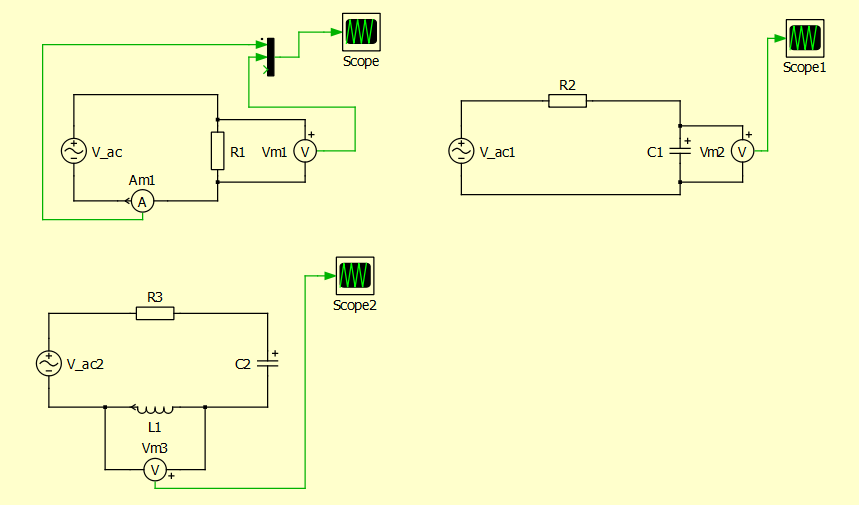
\includegraphics[width=1\textwidth]{Vildledning/Schematics/Eks1_LCR.png}
	\caption{LCR-Kredsløb}
	\label{forslag1}
\end{figure}

Hvor:
\begin{table}[H]
	\begin{tabular}{l|l}
	$R$     & Resistans [\si \ohm] \\
	$V_{ac}$ 	   &  Generator[\si Volt] \\
	$A$ 	   & Ampere-meter [\si Ampere] \\
	$V$			& Volt-meter [\si Volt]
	\end{tabular}
\end{table}

\newpage
